\section{Recovery of periods from {\harps} data}
\protect\label{section:harpsper}

Attempts to derive periodograms from the results of the the various measures listed in Section \ref{section:linemeas}
met with much less success than the photometric results from {\asas} and {\hst}, in that, as discussed in Appendix
\ref{chapter:lsroutines}, all the various Lomb-Scargle routines gave very different results for almost every line
measure or combination of measures. A full list of results is \examrevision{not listed in this \paperorthesis, however
  the overall performance is illustrated in Fig. \ref{fig:photcomp1} and Fig. \ref{fig:photcomp2} in Section
  \ref{section:asasfap}.} The {\numrecs} routine usually failed to find periods close to the 82.6 day period identified
in the photometric results or on the occasions when it found it, gave a FAP at or very close to 1.0.

To examine the performance as well as possible, all the three Python routines described in Appendix
\ref{chapter:lsroutines} were tried with every set of data and the results compared. None of the routines gave any
meaningful results for \examrevision{periods} below 40 days, with a plethora of strong peaks down to fractions of a day,
or above 120 to 130 days, so all the periodograms were generated with periods between 40 and 130 days, in steps of 0.01
days (14 minutes, 20 seconds). This encompassed the 41.3 days of \citet{benedict93}, although this looks very likely to
be a half-period \examrevision{sub-harmonic}, through to and including the 116.6 days of \citet[Table
3]{suarezmascareno15} and encompassing the minimum period of 50 days given by \citet{kurster99} and the 82 days of
\citealt{benedict92,benedict98,kiraga07}. The erratic behaviour of the periodograms below about 40 days made it
impractical to extend the search down to include the 31.5 days of \citet{guinan96}, but in the light of the photometric
results and the unanimity of other reports as to the period being longer than this, this was deemed not to matter.

Many of the periodograms showed several strong peaks all over the range searched, typically with up to five outstanding
peaks in the range searched, so for this {\paperorthesis} note was taken of the periods of the strongest peaks and of
the five strongest peaks in the analyses of the periodograms.

In Fig. \ref{fig:harpspgrams1} is shown how the different routines give different results with identical data; the upper
panel showing the results from the {\astroml} routine and the lower panel showing the results from {\gatspy}. In
Fig. \ref{fig:harpspgrams2} is shown a result from peak ratio calculation giving a value of 82.2 days returned by
\gatspy.

\begin{figure}[!htbp]
\begin{center}
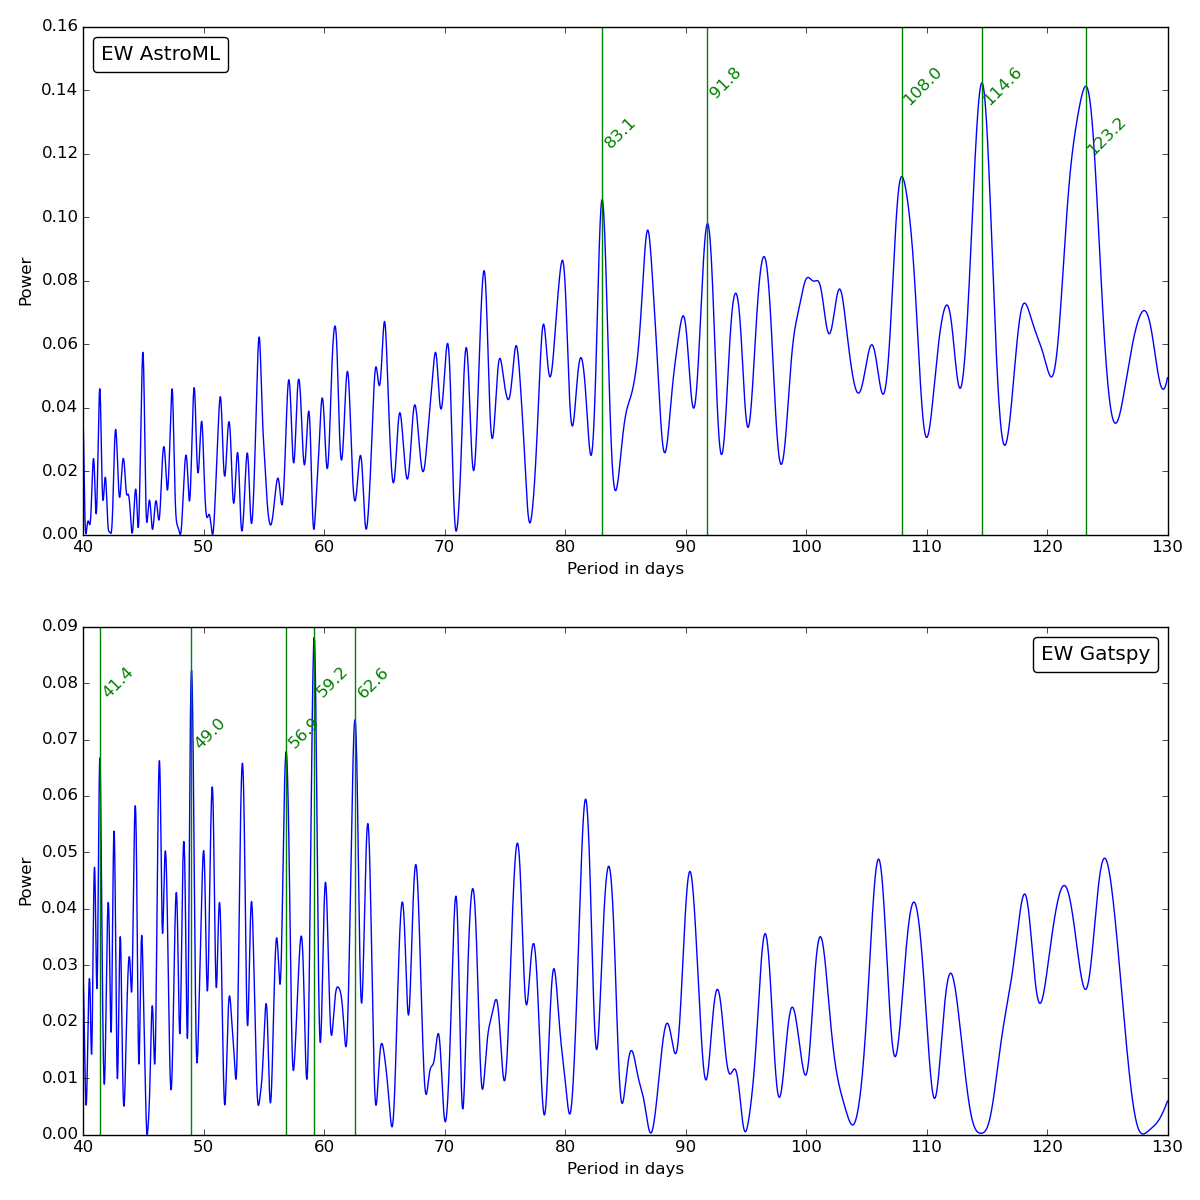
\includegraphics[scale=0.35]{Figures/summpgrams.png} \\
\end{center}   
\caption{This figure shows sample periodograms from the {\ha} peak of the {\harps} data, calculating from equivalent
  widths using {\astroml} for the upper panel and {\gatspy} for the lower panel. The strongest 5 peaks are highlighted
  in both cases.}
\protect\label{fig:harpspgrams1}
\end{figure}

\begin{figure}[!htbp]
\begin{center}
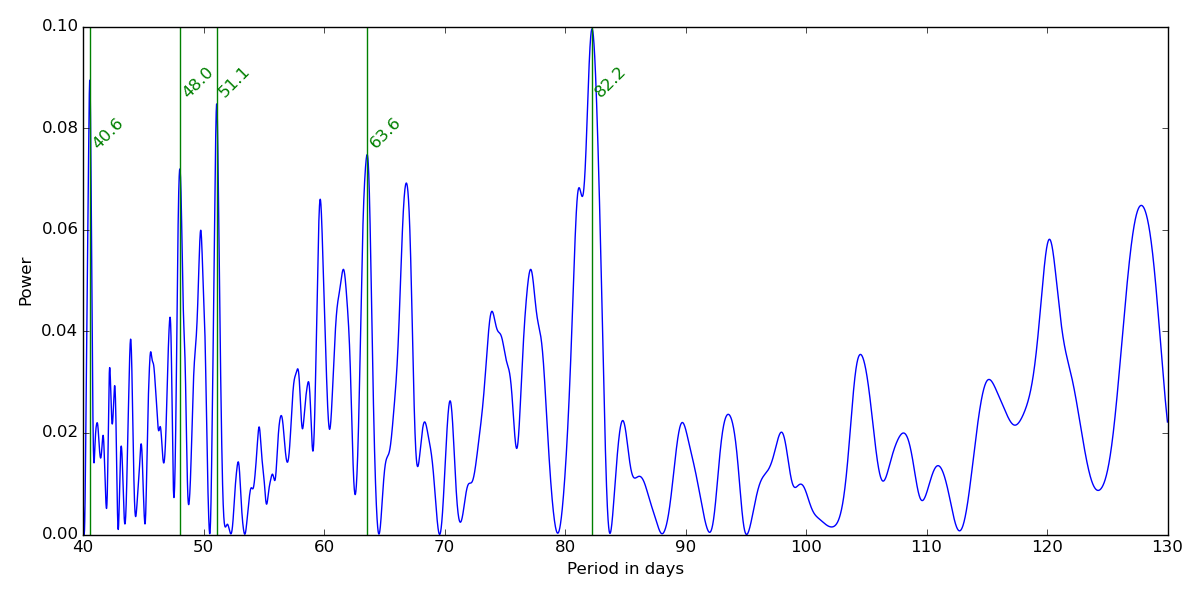
\includegraphics[scale=0.40]{Figures/harpsprbind1.png} \\
\end{center}   
\caption{This figure shows a sample periodogram from the peak ratio measure from the Full Set of the data from {\harps}
  binned to 1 day, processed by the {\gatspy} routine and displayed with the five highest peaks highlighted and showing
  the values. \Notnow{This corresponds to the ninth row Table \ref{table:fullprtaball}.}}
\protect\label{fig:harpspgrams2}
\end{figure}

Some efforts were made to remove data contaminated from flares, either by clipping spectra with various upper bounds of
equivalent width, by binning data or both. Following the lead from {\uves} in Section \ref{section:uvesflares}, spectra
were clipped where the equivalent width exceeded one standard deviation from the median. This was 3.8{\AA} for the
Original Set or 4.2{\AA} for the Full Set of data. However the latter, which included some spectra with very large
equivalent widths taken in 2016, did not yield any particular benefit, so with the Full Set of data, clipping to a
maximum equivalent width of 3.8{\AA} in line with the Original Set was tried. \examrevision{Binning to various fractions
  of a day up to one day was attempted.  Nothing was observed to improve the performance of any of the measurements in
  any consistent way, with the possible exception of peak ratios, which appeared to improve very slightly if binned to
  around 1 day. The results from the {\ha} Index were virtually identical to those from the equivalent width measure, so
  these are not considered separately. The overall performance of the four methods is summarised and illustrated in
  Fig. \ref{fig:photcomp1} and Fig. \ref{fig:photcomp2}.}

\examrevision{With the Original Set of data, all the measurements, except for the peak ratio, returned the 116.6-day
  period reported in \citet[Table 3]{suarezmascareno15}. This completely disappeared if any clipping or binning was done
  or the Full Set of data was examined. The window function of both these sets of observation times are shown in
  Fig. \ref{fig:harpswfos} and Fig. \ref{fig:harpswffs}. It can be seen that \examrevisiona{peaks close to this can be
    found in the window function for the Original Set}, suggesting this as the cause of the 116-day period in
  periodograms derived from this data.}

\begin{figure}[!htbp]
\begin{center}
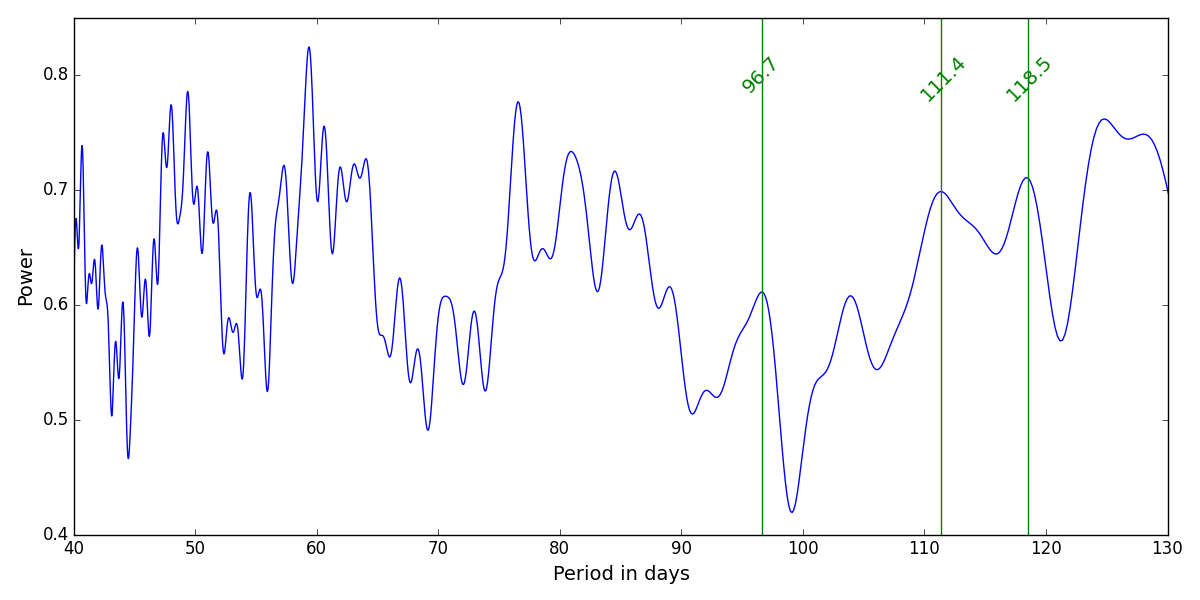
\includegraphics[scale=0.45]{Figures/harpswfos.png} \\
\end{center}   
\caption{\examrevision{Window function of Original Set of {\harps} data (observation times up to January 2014), with
    peaks highlighted in the area of 90 to 130 days, showing peaks \examrevisiona{either side of 116.6 days}, which appeared in several of the
    periodograms (for all measurements except peak ratio).}}
\protect\label{fig:harpswfos}
\end{figure}

\begin{figure}[!htbp]
\begin{center}
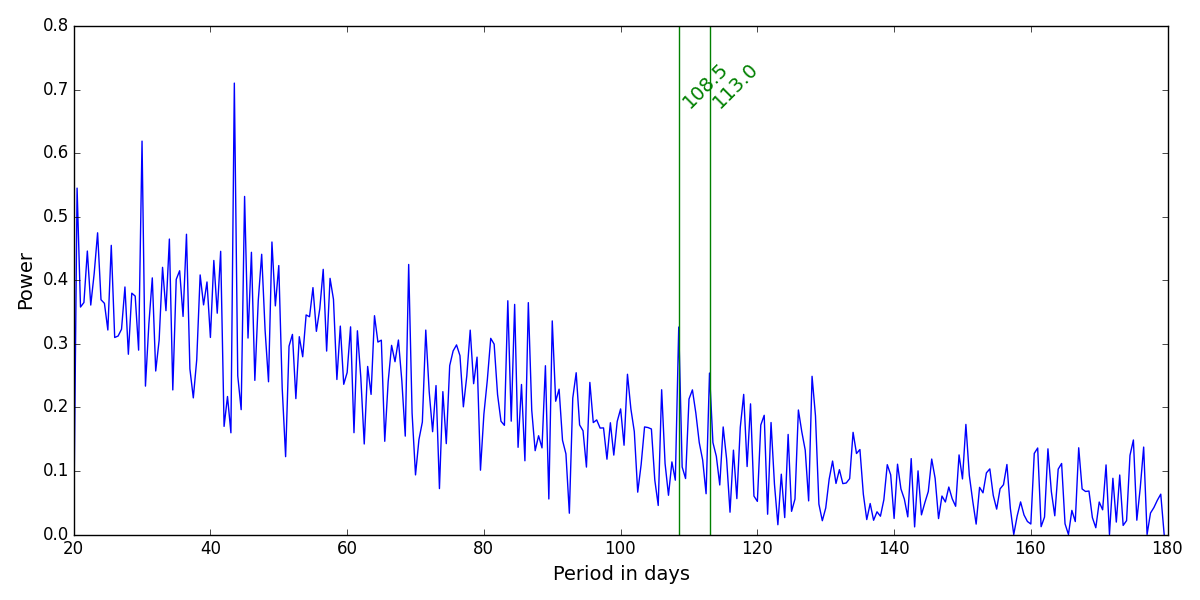
\includegraphics[scale=0.45]{Figures/harpswffs.png} \\
\end{center}   
\caption{\examrevision{Window function of Full Set of {\harps} data (observation times up to March 2016), with
    peaks highlighted in the area of 100 to 130 days. In this case there \examrevisiona{were no peaks close to 116.6 days} as observed in
    Fig. \ref{fig:harpswfos}.}}
\protect\label{fig:harpswffs}
\end{figure}
